%\chapter{Appendix B: QTOR}
\chapter{Miscellaneous}
\label{Miscellaneous}

%%%%%%%%%%%%%%%%%%%%%%%%%%%%%%%%%%%%%%%%%%%%%%%%%%%%%%%%%%%%%
\section{Target BPM Angle Resolution}
\label{Target BPM Angle Resolution 2}

%The objective is to estimate the effective target angle resolution using a position
%measurement at a upstream BPM.
%* Ideally want to find a model location where angle jitter at the target
%corresponds to pure position at the upstream BPM.
%* With known BPM position resolution, effective target angle resolution can be
%estimated.
%
%Target angle resolution using 3P02A is better than the angle resolution we
%have now.
%
%Incorporating BPM 3P02A into a regression scheme might be a good idea.
%
%Note: A study of strength sharing between angle and position in the various BPM's
%along the beamline (similar to Don's study at ELOG 856) for wien0 (two runs from
%each slug) seems to show Compton BPMs (3P02A \& B) were insensitive to
%position on target.
%
%
%OPTIM confirms that the Compton region should have appropriate optics
%for UVA?s angle-sensitive BPM (i.e. angle jitter at the target is transformed
%to position jitter at the BPM).
%
%* With X (Y) BPM position resolution of 0.90 (0.96) ?m, the effective target
%angle resolution is estimated to be 0.048 (0.060) ?rad. This is better than
%the angle resolution we have now, so we encourage UVA?s strategy of
%incorporating this BPM into a regression scheme.



\begin{singlespace}
\begin{figure}[!h]
	\begin{center}
	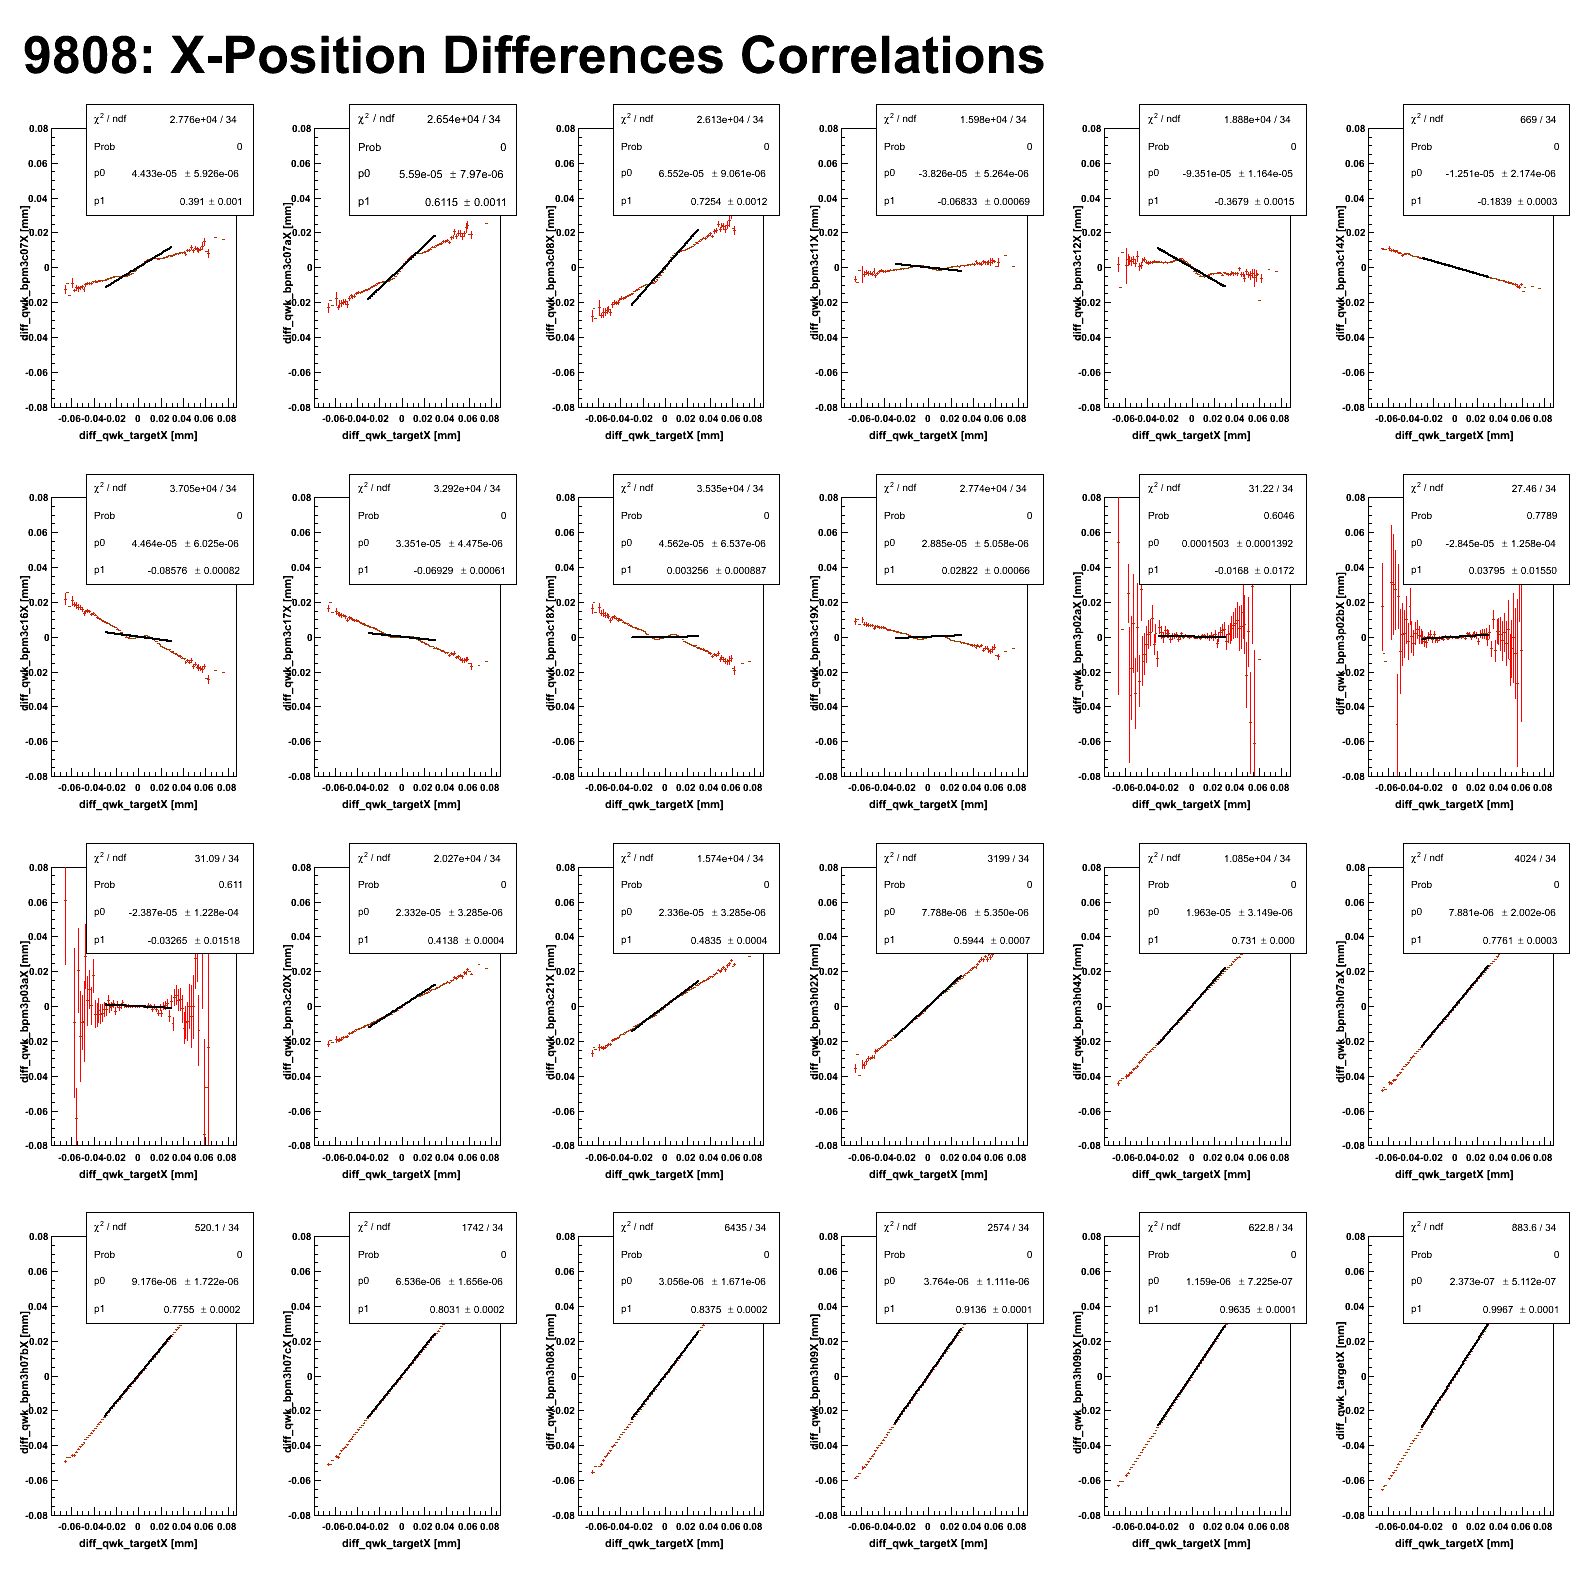
\includegraphics[width=15.0cm]{figures/XtgtCorrelation9808}
	\end{center}
	\caption
%	[The BPM target X correlation with other upstream BPMs for a run during Wien 0.]
	{The BPM target X correlation with other upstream BPMs for a run during Wien 0.}
	\label{fig:XtgtCorrelation9808}
\end{figure}
\end{singlespace}

\begin{singlespace}
\begin{figure}[!h]
	\begin{center}
	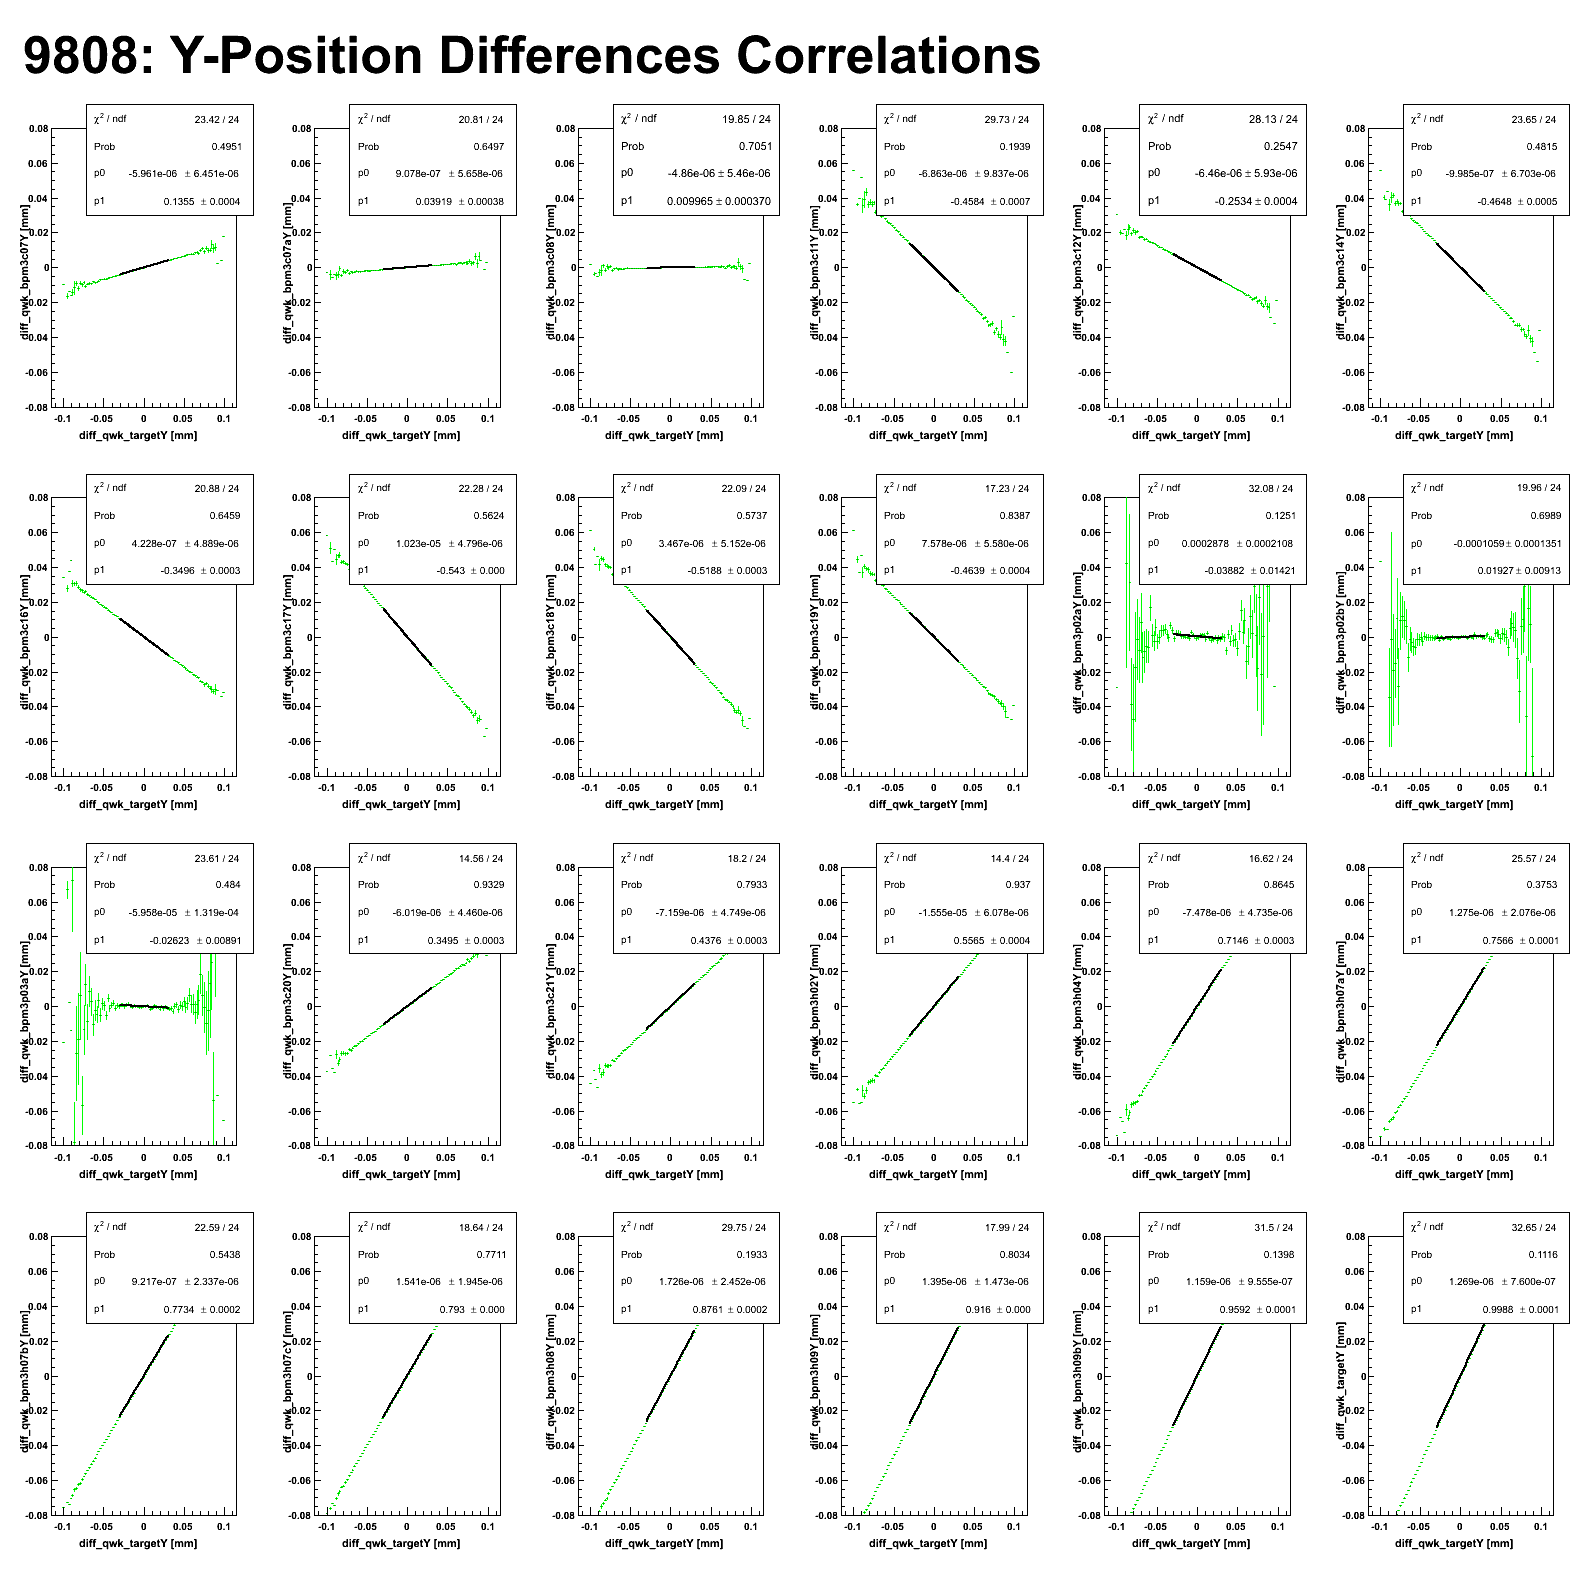
\includegraphics[width=15.0cm]{figures/YtgtCorrelation9808}
	\end{center}
	\caption
%	[The BPM target Y correlation with other upstream BPMs for a run during Wien 0.]
	{The BPM target Y correlation with other upstream BPMs for a run during Wien 0.}
	\label{fig:XtgtCorrelation9808}
\end{figure}
\end{singlespace}



%%%%%%%%%%%%%%%%%%%%%%%%%%%%%%%%%%%%%%%%%%%%%%%%%%%%%%%%%%%%%
\section{Regression Independent Variable Correlation}
\label{Relative Weighted Yield Stability for Q-weak}


\begin{singlespace}
\begin{figure}[!h]
	\begin{center}
	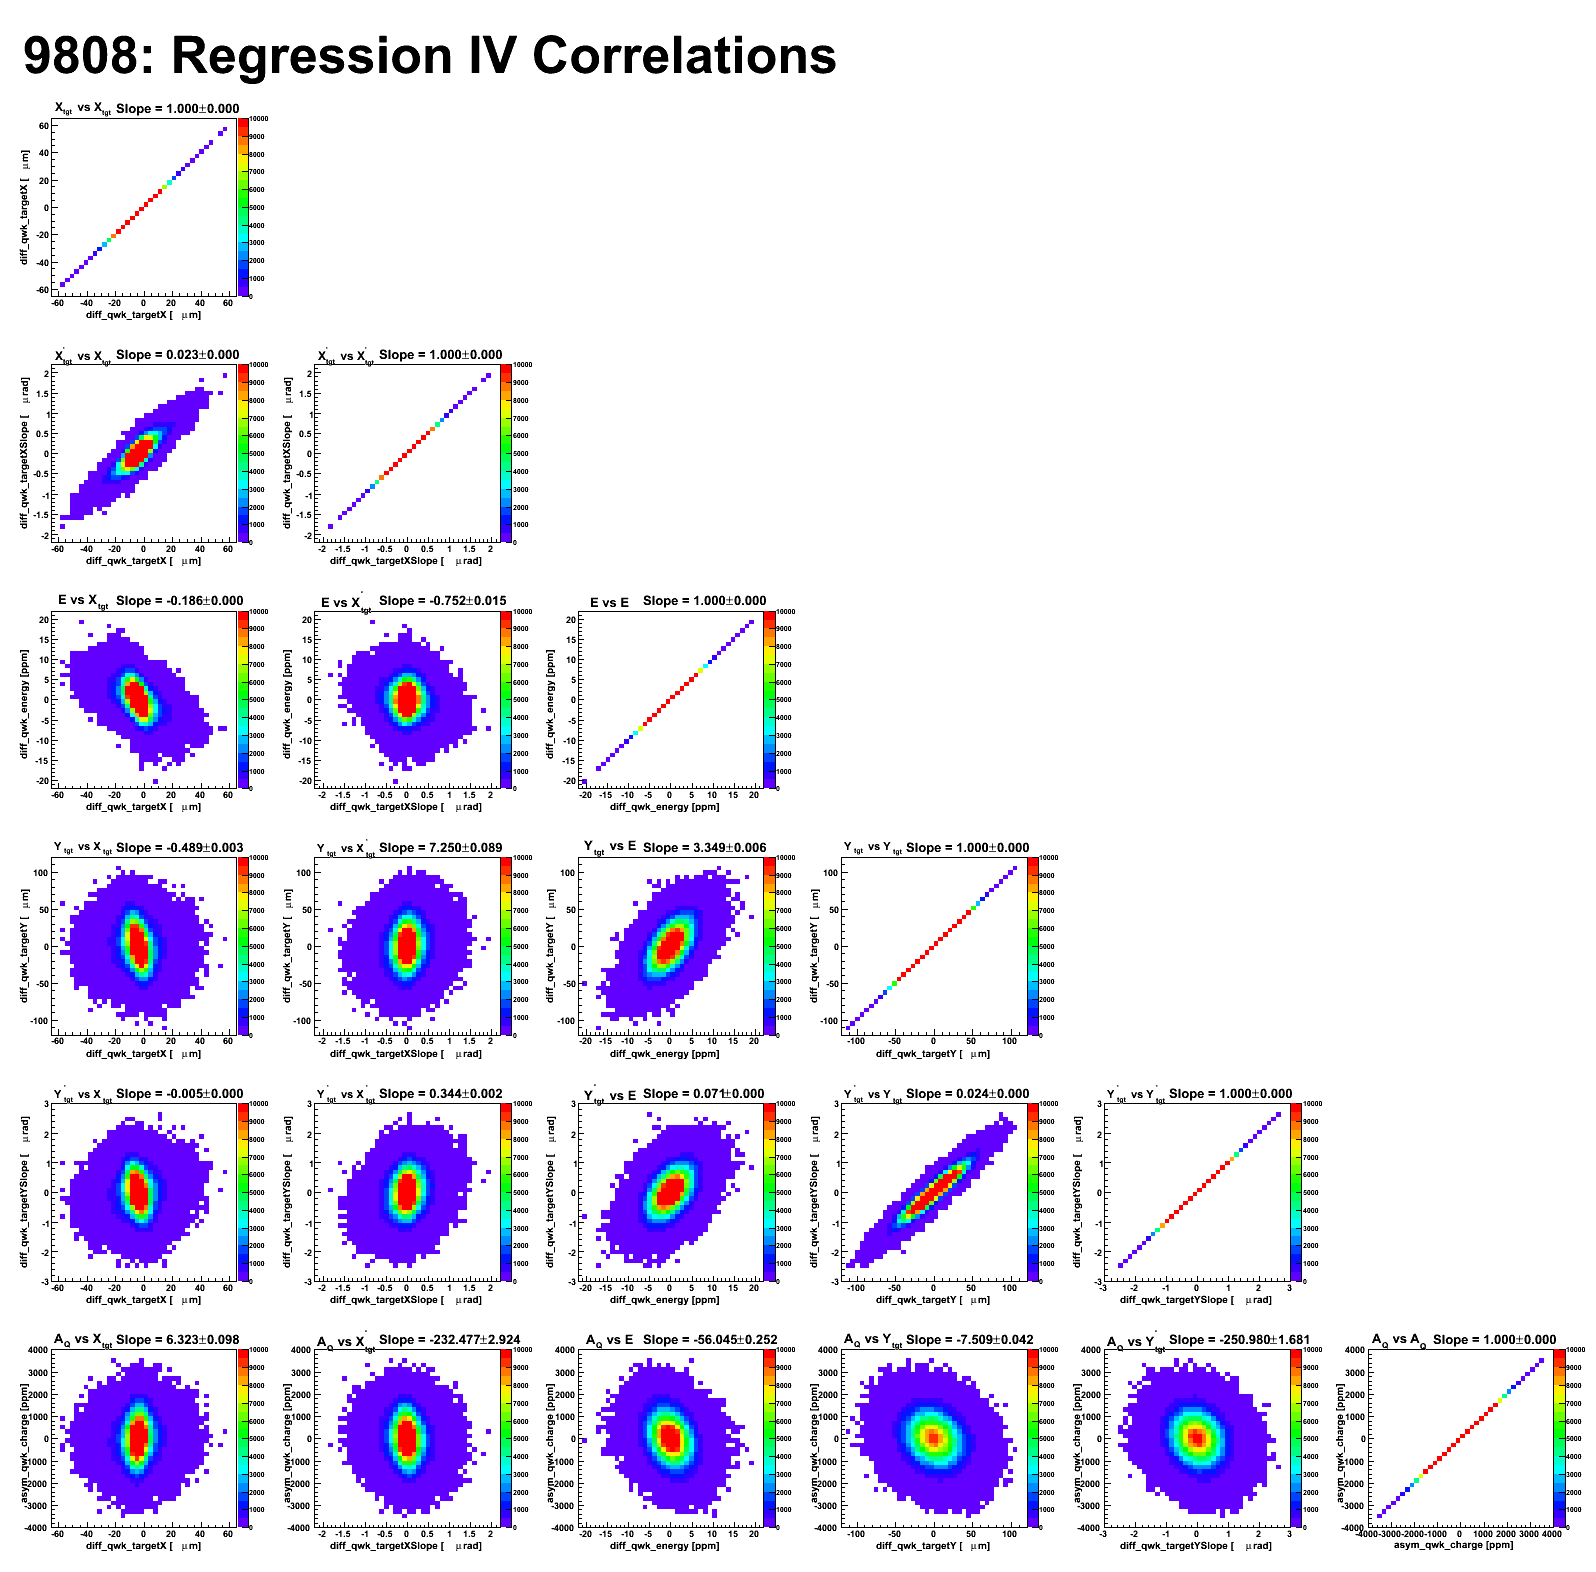
\includegraphics[width=15.0cm]{figures/regIV_correlationWien0}
	\end{center}
	\caption
%	[The correlation between regression variables for a run during Wien 0.]
	{The correlation between regression variables for a run during Wien 0.}
	\label{fig:regIV_correlationWien0}
\end{figure}
\end{singlespace}

\begin{singlespace}
\begin{figure}[!h]
	\begin{center}
	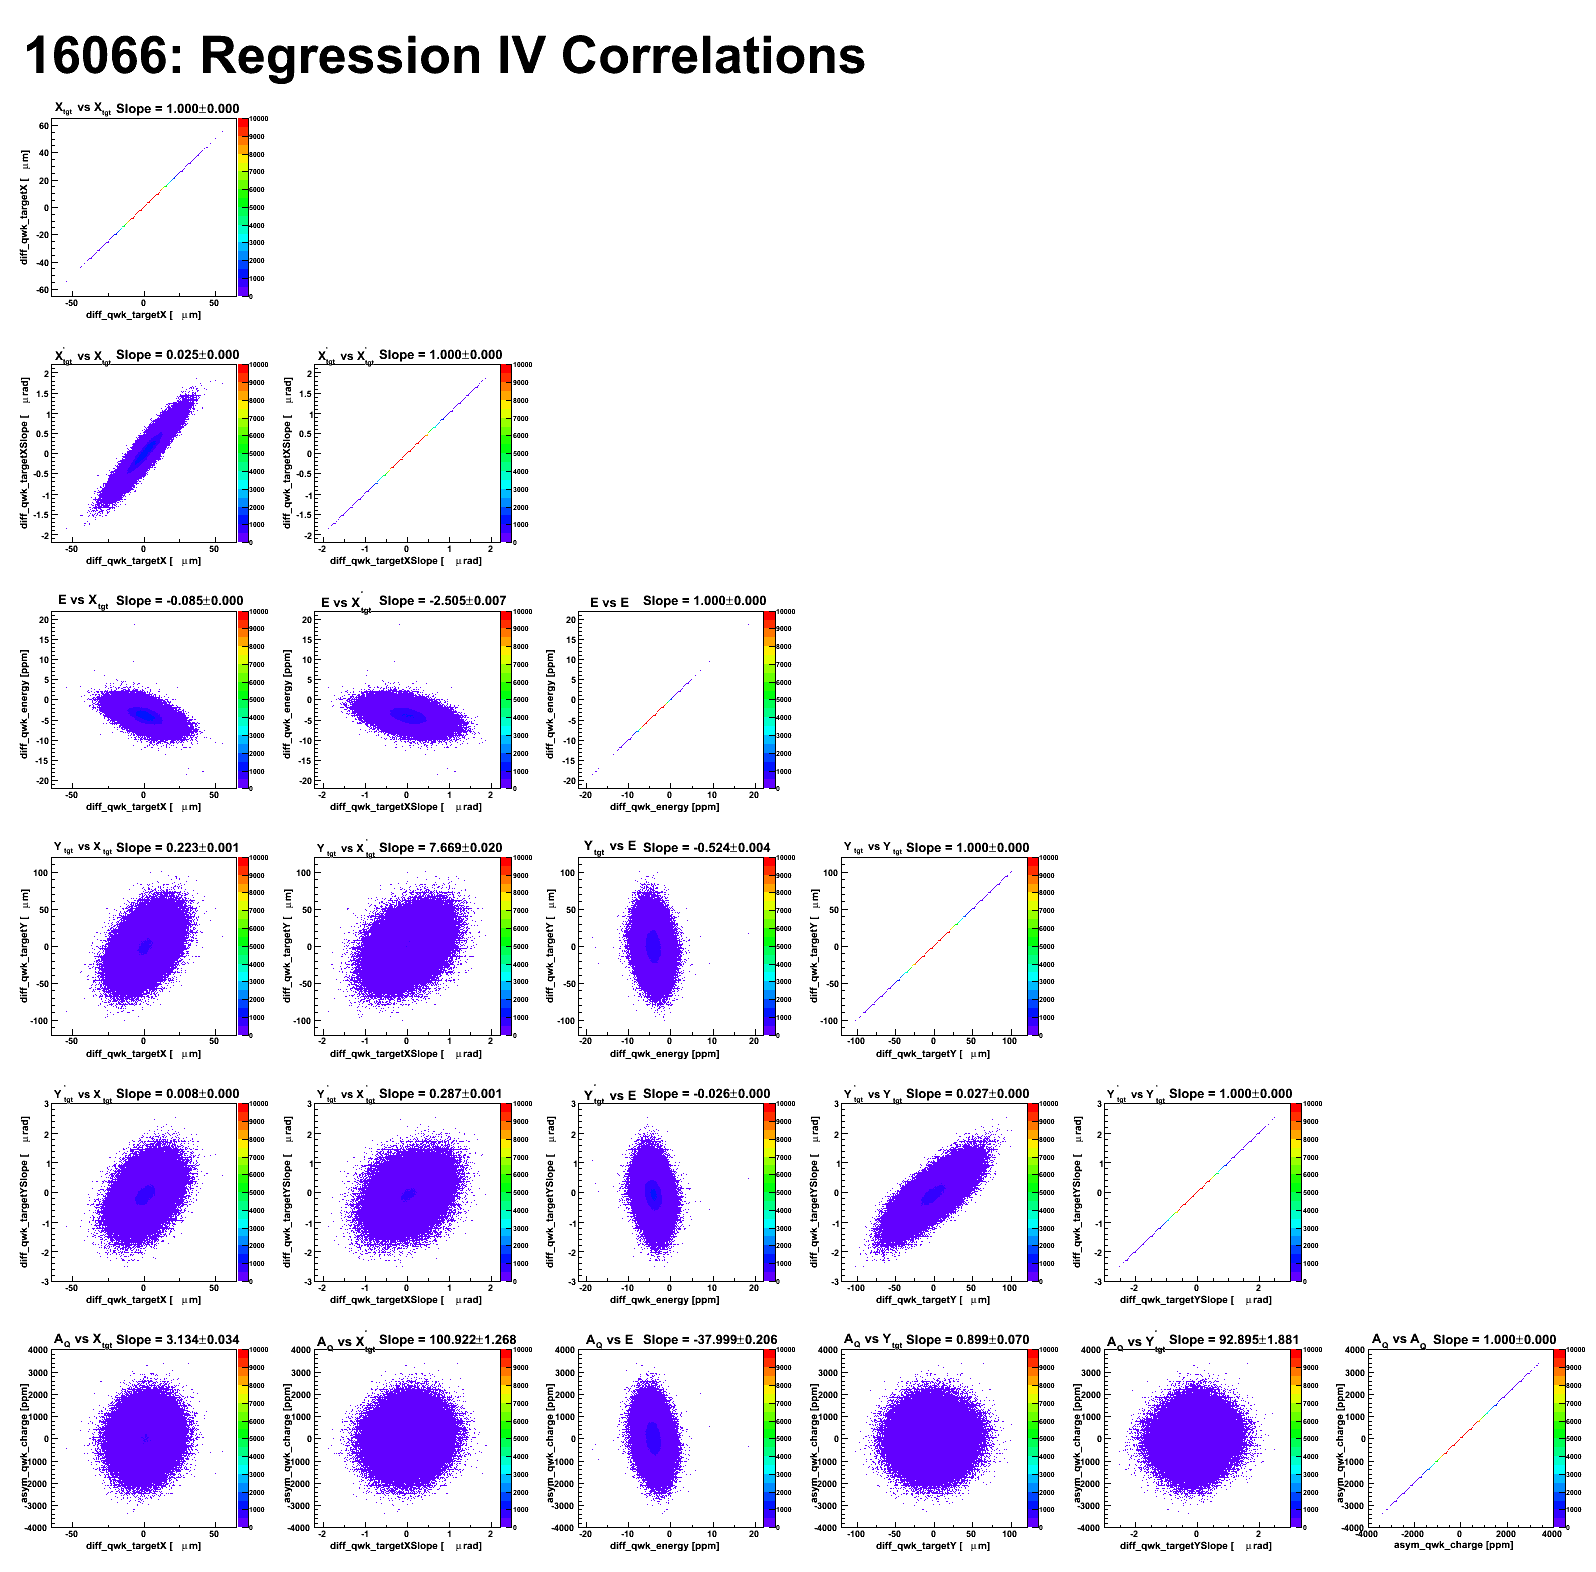
\includegraphics[width=15.0cm]{figures/regIV_correlationRun2}
	\end{center}
	\caption
%	[The correlation between regression variables for a run during Run 2.]
	{The correlation between regression variables for a run during Run 2.}
	\label{fig:regIV_correlationRun2}
\end{figure}
\end{singlespace}





%%%%%%%%%%%%%%%%%%%%%%%%%%%%%%%%%%%%%%%%%%%%%%%%%%%%%%%%%%%%%
\section{Relative Weighted Yield Stability for Q-weak}
\label{Relative Weighted Yield Stability for Q-weak}

\begin{singlespace}
\begin{figure}[!h]
	\begin{center}
	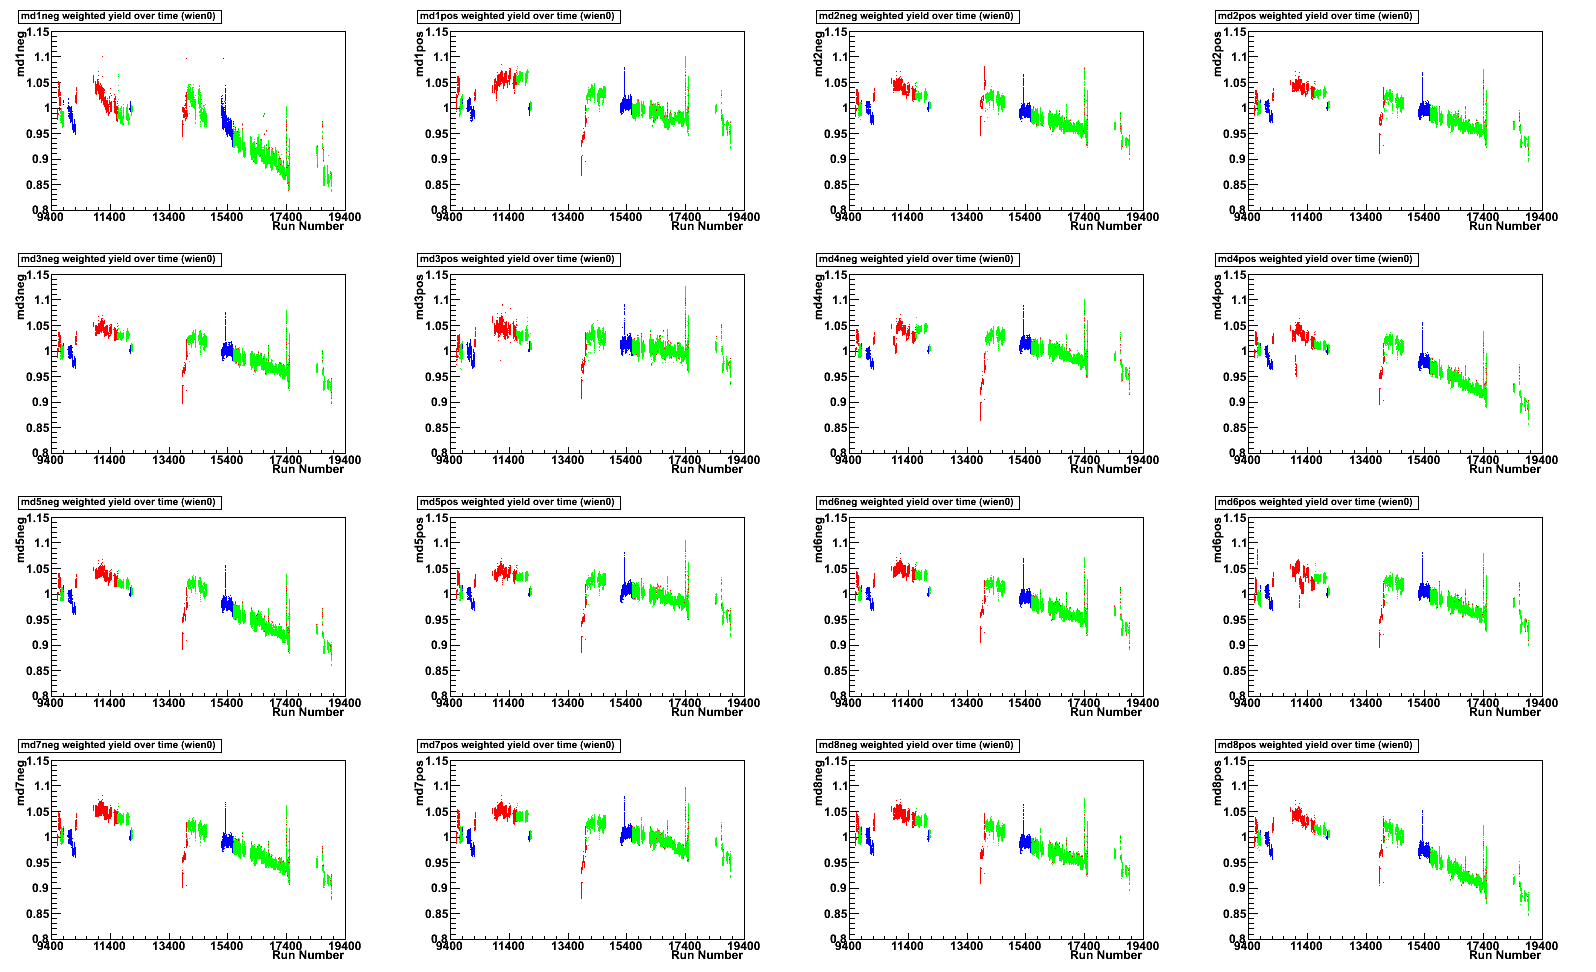
\includegraphics[width=15.0cm]{figures/qweakPVweightedYield}
	\end{center}
	\caption
%	[The weighted yield for each PMT tube in the main detector.]
	{The weighted yield for each PMT tube in the main detector and can be expressed as $w_{i} \times Y_{i} = Y_{i}/<Y_{i}>$. Ideally expect to be equal to 1. The weights are equal to the yields at about the 5\% level for run1. One can see drifts during Run 2. Each data point is a runlet and the plot was made using the database rootfiles. The weights used for a given runlet to calculate the relative weighted yield are those appropriate for that time based on the mapfile names.}
	\label{fig:qweakPVweightedYield}
\end{figure}
\end{singlespace}

\begin{singlespace}
\begin{figure}[!h]
	\begin{center}
	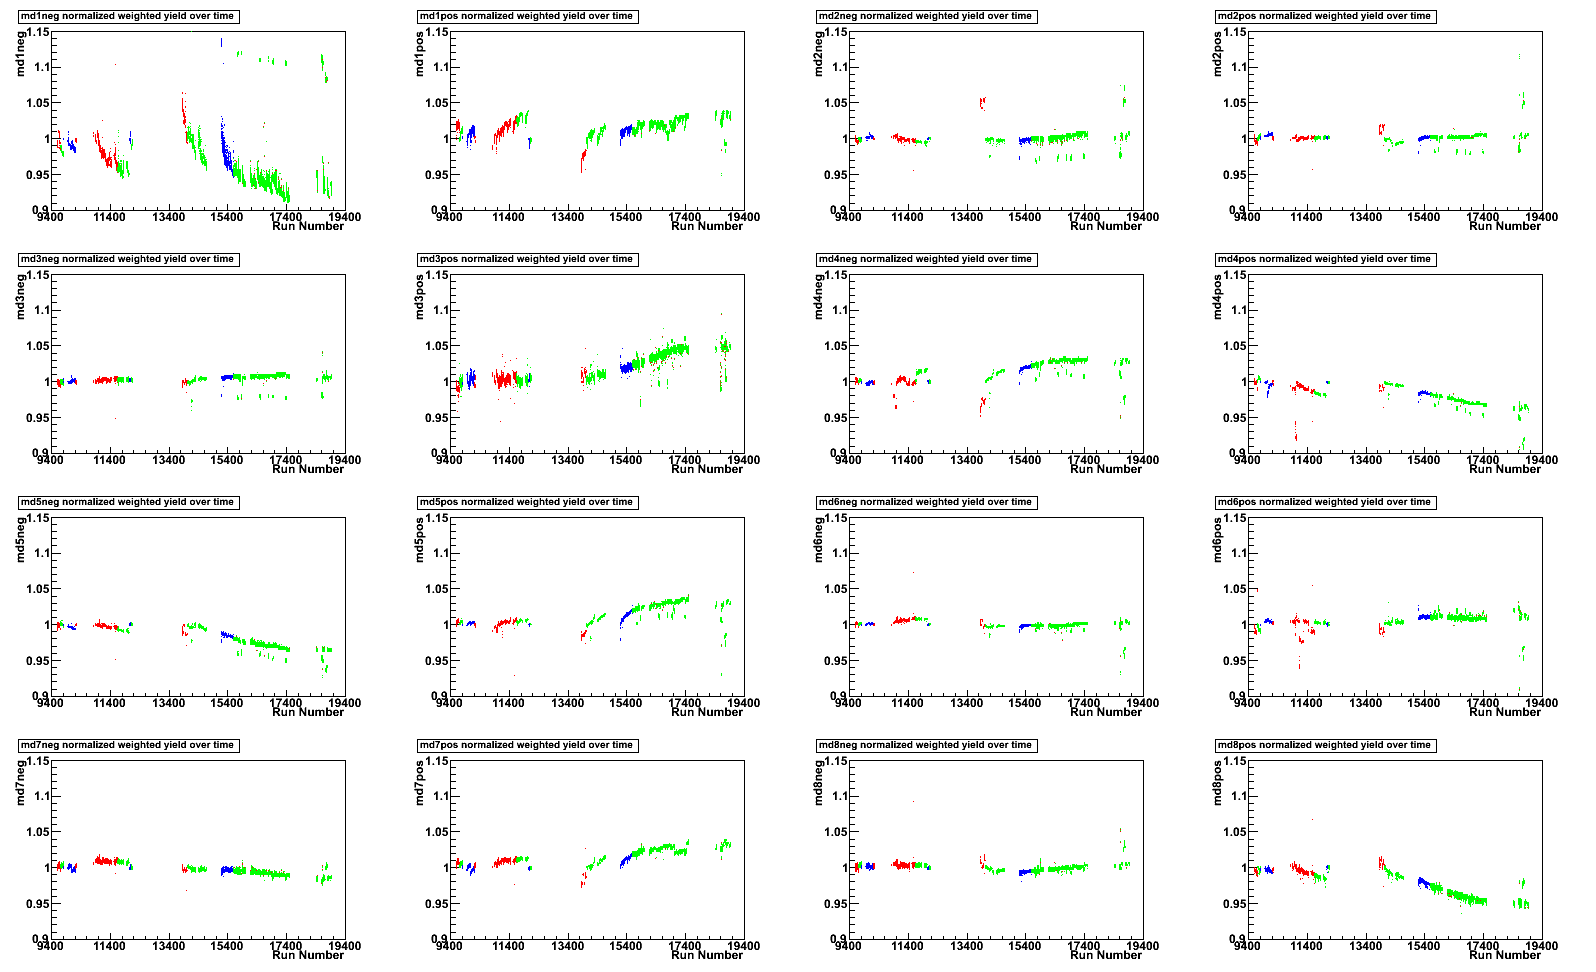
\includegraphics[width=15.0cm]{figures/qweakPVrelWeightedYield}
	\end{center}
	\caption
%	[The relative weighted yield for each PMT tube in the main detector.]
	{The relative weighted yield for each PMT tube in the main detector and can be expressed as $w_{i} \times Y_{i}/ \sum(w_{i} \times Y_{i}/16)$. Color transitions mark the beginning of a weighting period defined by the mapfiles.}
	\label{fig:qweakPVrelWeightedYield}
\end{figure}
\end{singlespace}
